\documentclass[a4paper,12.5pt]{scrreprt}
\usepackage[utf8]{inputenc}
\usepackage[T1]{fontenc}
\usepackage[english]{babel}		% English language 
%--------------------------------------------------
% font and formatting
\usepackage{lmodern}					% font looks better on screen
\usepackage{microtype}				% even better
\usepackage{fullpage}					% more space on the page
\usepackage{natbib}
%--------------------------------------------------
% more features
\usepackage{amsmath}					% all the fancy math stuff
\usepackage{listings}         % code listings
\usepackage{enumerate}				% customize numbered lists
\usepackage{paralist}					% inline lists
\usepackage{graphicx}					% fancy graphics
\usepackage{color}						% enable color
\usepackage{xspace}						% to space or not to space...
\usepackage{url}							% URL handling
\usepackage{hyperref} 				% should be loaded last
%--------------------------------------------------

% setup natbib citation format
\bibpunct{(}{)}{,}{a}{,}{,}

% setup the listings package
\lstset{%
	language=perl,
	basicstyle=,                       % the size of the fonts that are used for the code
	numbers=left,                      % where to put the line-numbers
	numberstyle=\tiny,                 % the size of the fonts that are used for the line-numbers
	%stepnumber=2,                      % the step between two line-numbers. If it is 1 each line will be numbered
	numbersep=5pt,                     % how far the line numbers are from the code
	backgroundcolor=\color{lightgrey}, % choose the background color. You must add \usepackage{color}
	showspaces=false,                  % show spaces adding particular underscores
	showstringspaces=false,            % underline spaces within strings
	showtabs=false,                    % show tabs 
	frame=none,                        % can be: none, leftline, topline, bottomline, lines, single, shadowbox 
	%frameround=tttt,                   % rounded corners; t=round, f=corner
	tabsize=2,                         % sets default tabsize to 2 spaces
	captionpos=t,                      % caption position (t|b)
	breaklines=true,                   % automatic line breaking
	breakatwhitespace=false,           % automatic breaks should not happen at whitespace
	%escapeinside={\%}{)}               % if you want to add a comment within your code
}

% setup hyperlinks, bookmarks and pdf metadata
\hypersetup{%
	bookmarks=true,
	linktocpage=true,
	pdftitle={Fast and efficient mapping of transcript sequences to ortholog groups},
	pdfauthor={Malte Petersen},
	pdfcreator={pdflatex},
	pdfsubject={orthology prediction},
	pdfkeywords={orthology} {prediction} {est} {transcriptome} {phylogeny} {thesis}
}

% new colors and commands
\definecolor{lightgrey}{rgb}{0.9,0.9,0.9}
\newcommand{\file}[1]{{\lstinline{#1}}}
\newcommand{\code}[1]{{\texttt{#1}}}
\newcommand{\hamstr}{HaMStR\xspace}
\newcommand{\pname}{Orthograph\xspace}
\newcommand{\species}[1]{\textit{#1}}
\newcommand{\todo}[1]{\textbf{\color{red}[#1]}}

% doublespace
\linespread{1.3}

\title{Fast and efficient mapping of transcript sequences to ortholog groups}
\author{Malte Petersen}

\begin{document}
\maketitle
\tableofcontents

\chapter*{Paper notes}
	\todo{where do I put hmmtest?}

Strategies for orthology prediction:

Tree reconciliation

\begin{itemize}
	\item topology of a gene tree compared with that of the chosen species tree
	\item reconciled by maximum parsimony $\rightarrow$ reflects ortholog
		relationships
	\item genome-wide application precluded by:
	\begin{itemize}
		\item horizontal gene transfer, especially in prokaryotes (widespread HGT
			invalidates the very notion of a species tree)
		\item computationally expensive
	\end{itemize}
\end{itemize}

\begin{description}
	\item[\cite{mirkin1995}] Tree-based approach to orthology prediction
	\item[\cite{page1998}] Tree reconciliation method
	\item[\cite{yuan1998}] Tree-based approach to orthology prediction
	\item[\cite{kuzniar2008}] Review of approaches
\end{description}

most studies employ simplifications/shortcuts $\rightarrow$ graph-based approaches:

Triangulation

\begin{itemize}
	\item OrthoDB 
	\item COG (KOG, EGO, etc)
\end{itemize}

Reciprocal best hit (RBH) 

\begin{itemize}
	\item RBH strategies recover only one-to-one orthologs (the bidirectional best
		hit)
	\item InParanoid (BLAST based)
\end{itemize}

Markov clustering:

\begin{itemize}
	\item OrthoMCL
\end{itemize}

Homoplasy: similarity in unrelated organisms. Homoplasies demonstrate adaptation
in the living world.

Homoplasy \citep{lankester1870}: It may be said that the term ``analogy'',
already in use, is sufficient to indicate what is here termed ``homoplasy''; but
analogy has had a wider signification given to it, in which it is found very
useful to employ it, and if could not be used with any accuracy in place of
homoplasy.  \emph{Any} two organs having the same function are analogous,
whether closely resembling each other in their structure and relation to other
parts or not, and it is well to retain the word in that wide sense. Homoplasy
includes all cases of close resemblance of form which are not traceable to
homogeny, all \emph{details} of agreement not homogenous, in structures which
are broadly homogenous, as well as in structures having no genetic affinity.


%\mainmatter
%\chapter{Journal}
	%\section{August - November 2011}
\subsection*{2011-08-15 Treffen mit Oliver/Karen}

\begin{figure}[h]
	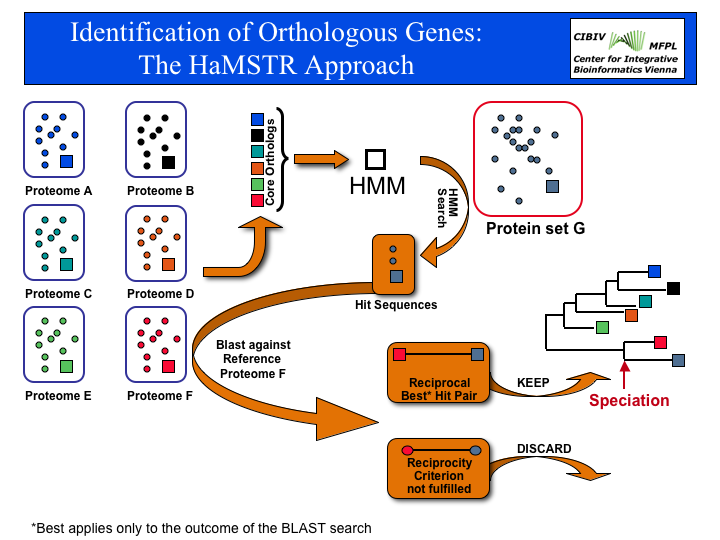
\includegraphics[width=\textwidth]{img/hamstr-schema.png}
	\caption{\cite{Ebersberger2009}}
\end{figure}

Tasks:

\begin{itemize}
	\item read paper
	\item install HaMStR, test
	\item read \& understand the source:
		\begin{itemize}
			\item what is happening when
			\item at what point does it use genewise?
		\end{itemize}
	\item look up:
		\begin{itemize}
		\item genewise/exonerate (alignment NA $\rightarrow$ AA)
			\item PAL2NAL
			\item ESTwiseDB
			\item BLASTx (what does it do)
		\end{itemize}
\end{itemize}

Vortrag beim Montagskolloquium über DA (desinteressiertes, ahnungsloses
Publikum)

\begin{itemize}
	\item Warum?
\end{itemize}

\subsection*{2011-08-16}

Installed HaMStR v8 with all dependencies:

\begin{table}[h]
	\begin{tabular}{l l l}
		\textbf{Package} & \textbf{Version} & \textbf{Source}\\
		\hline
		HMMer    & 3.0	 & http://www.deep-phylogeny.org/hamstr/download/ \\
		ClustalW & 2.1   & ftp://ftp.ebi.ac.uk/pub/software/unix/wise2/ \\
		Genewise & 2.2.0 & http://hmmer.janelia.org/software \\
	\end{tabular}
\end{table}

All programs were installed in PATH. With Genewise, a modification was
necessary in \file{src/HMMer2/sqio.c}: renamed getline() to genewise\_getline()
since getline() is already defined in \file{stdio.h} (standard C library).

All test runs according to the README files were successful.

Read the HaMStR paper (\cite{Ebersberger2009}).

Tried to get an insurance for the lab key, so far unsuccessful.

\subsection*{2011-08-17}

Picked up playground data and annotations from Karen.

\subsection*{2011-08-18 What does HaMStR do?}

Genewise: At the very end, \emph{after} the re-BLAST. Translates ESTs to
revcomp, only if at least one hit was obtained.

\subsection*{2011-08-23 Karen}

\begin{itemize}
	\item ``transitive closure'' $\rightarrow$ lookup \url{deep-phylogeny.org}
	\item InParanoid: Orthology by pairwise assignment
	\item OrthoMCL: Orthology by pairwise $\rightarrow$ groups of orthologs. Read
		presentations.
	\item parallelize: spawn daughter processes according to \#CPU?
\end{itemize}

\subsection*{2011-08-24 Oliver}

``deep search'': blast instead of hmmsearch (weniger sensitiv)

``very deep search'': hmm hits mit estwisedb (übersetzen und suchen in 1) gegen
core-orthologs

Warum nur orthologe Gene durchsuchen? $\rightarrow$ auch nicht orthologe,
vielleicht passen sie besser.

EST-Set schrittweise verkleinern\dots

Benchmarks mit absichtlich verschlechterten Sequenzen, z.B. einen von den
Core-Orthologen zufällig verändern.

\begin{table}
	\begin{tabular}{l l}
	\textbf{program} & \textbf{compares} \\
	\hline
	genewise   & single protein vs single DNA seq \\
	genewisedb & protein database vs DNA database \\
	estwise    & single protein vs single EST/cDNA seq \\
	estwisedb  & protein database vs EST/cDNA database
	\end{tabular}
\end{table}

valid command line:
\begin{verbatim}
../hamstrsearch_local-hmmer3.v8.pl
-sequence_file=cleaned/Adelphocoris_lineolatus_contig.fa
-fasta_file=ortholog_set_insecta_hmmer3-1/insecta_hmmer3-1.fa -taxon=apime
-refspec=dappu_1391 -blast_path=ortholog_set_insecta_hmmer3-1/blast_dir -est
\end{verbatim}

\section{September 2011}
\subsection*{2011-09-02}

Karen nach Erklärung fragen:
\renewcommand{\labelenumi}{\alph{enumi})}
\begin{enumerate}
	\item Frameshifts + deren Korrektur
	\item Introns + interne Stopcodons: Wie erkennen und sinnvoll entfernen?
\end{enumerate}

\includegraphics[width=0.5\textwidth]{img/hamstr-cmdline-files.pdf}
\begin{table}[h]
\begin{tabular}{l l l}
	\textcircled{A} & cleaned/Adelphocoris\_lineolatus\_contig.fa & $\leftarrow$ EST file (fasta)\\
	\textcircled{B} & ortholog\_set\_insecta\_hmmer3-1/insecta\_hmmer3-1.fa & $\leftarrow$ Core ortholog set (fasta)\\
	\textcircled{C} & dappu\_1391 & $\leftarrow$ reference taxon, from the core set \\
	 \textcircled{D} & ortholog\_set\_insecta\_hmmer3-1/blast\_dir & $\leftarrow$ BLAST database for the re-BLAST
\end{tabular}
\end{table}

\subsection*{2011-09-05 $\rightarrow$ 11 Started writing FORAGE}

\textbf{F}ind \textbf{O}rthologs using \textbf{R}eciprocity \textbf{A}mong
\textbf{G}enes and \textbf{E}STs 

\begin{description}
\item[Forage, v.:] Durchsuchen, (nach Nahrung) suchen etc.
\end{description}

There are BioPerl modules for 
\begin{enumerate}
	\item translation to all 6 reading frames
	\item using HMMer
	\item using BLAST
	\item reading \& writing files
\end{enumerate}
(but Oliver and Bernhard think I should stay away from them)

\subsection*{Intranet}

\fbox{\lstinline{boutEST\&Protein!2011}}

\begin{tabular}[h]{l l}
	\url{svzfmksql03} & $\rightarrow$ Server \\
	\url{131.220.75.253} & ~\\
	\url{lpd://131.220.75.250/przfmk010} & PPD: Apple 12/640ps\\
	\url{przfmk010} & 2. Etage\\
	\url{przfmk09} & 1. Etage\\
	\url{domzfmk} & Domain\\
	\url{131.220.228.166} & Cluster (pwd zfmk)\\
	\url{131.220.228.163} & alter Cluster\\
\end{tabular}

VPN? $\rightarrow$ Christoph fragen

\begin{lstlisting}
smbclient -W DOMZFMK -U <username> //SVZFMKSQL03/Molekular-Labor
\end{lstlisting}

\verb|mount.cifs| in \file{fstab}:
\begin{lstlisting}
//svzfmksql03/molekularlabor/ /mnt/zfmknet cifs noauto,users,credentials=/path/to/credsfile 0 0
\end{lstlisting}

\subsection*{2011-09-14}

Fiddled around with BioPerl, tried to reproduce Hamstr

hmmfound nothing in Andrena\_vaga $\rightarrow$ can this be true? Double-check!

\vspace{1em}
\begin{minipage}{0.4\textwidth}
	\begin{itemize}
		\item Substitute Unix tools w/ builtin Perl functions, e.g. grep/sed
		\item Debugging
		\item InParanoid source?
		\item CC license
		\item ``Forage''
		\item Computer?
	\end{itemize}
\end{minipage}
\hfill
\begin{minipage}{0.5\textwidth}
\textbf{PRIORITÄTEN}
\renewcommand{\labelenumi}{\arabic{enumi}.}
	\begin{enumerate}
		\item Korrigierte Nucleotide-Seq zu den Amino-Alignments die Hamstr
		ausspuckt $\rightarrow$ genewise-output speichern und parsen $\rightarrow$ pal2nal,
		sonst exonerate $\rightarrow$ Gerrit fragen! Prob?
		\item Orthologen-Set erstellen
	\end{enumerate}
\url{(arthropods.)eugenes.org}
\end{minipage}

\subsection*{2011-09-15}

be paranoid about BioPerl

\subsection*{2011-09-27 after I got this lab journal back\dots}

how the data structure could look like in Forage:

\begin{verbatim}
             {EST ID}
                 |
                 v
{seq, matched_by_hmm, hmm_score}
\end{verbatim}

how the data structure looks like in Hamstr:
\begin{verbatim}
            {taxon}
               |
               v
{prot=>hmm-hit seq, ids=>hmmhits, refseq=>refspec-seq, refspec=>refspec}
\end{verbatim}

\subsection*{2011-09-28}

\begin{lstlisting}
	$gw->{gw}	# ref to array
	print join("\n", @$gw->{gw})	# "not an ARRAY reference" error
	my $out = $gw->{gw};
	print join("\n", @$out); # works -> WTF?
\end{lstlisting}

Solution: dereferencing done correctly: 
\begin{lstlisting}
	print join("\n", @{$gw->{gw}}
\end{lstlisting}

\begin{itemize}
	\item ursprüngliche, korrigierte Nuc-Sequenz fehlt im Hamstr-output
	\item steht in genewise-output?
	\item sonst exonerate
	\item testen was genewise ausspuckt, wenn seq.\ künstlich verändert
	$\rightarrow$ frameshift, zus.\ A etc
\end{itemize}

\subsection*{2011-09-30 genewise splittet bei frameshifts}

\subsection*{2011-09-X cluster access}

\url{mptersen@131.220.228.166} pwd \url{zfmk}

List of installed software: \url{131.220.75.250}

Queueing system:

\begin{table}[h]
	\begin{tabular}{l l l}
	\verb|qsub| & <bash script> & (multiple opts for the script\dots RTFM)\\
	\verb|qstat| & show running stuff & (\verb|-f| full output)\\
	\verb|qdel| & delete jobs & ~ \\
	\verb|qhost| & show running stuff & (\verb|-j| by all users)\\
	\verb|mpirun| & for MPI & $\rightarrow$ only where it makes sense, read docs
	first!
	\end{tabular}
\end{table}

important: no relative paths in scripts

\section{October 2011}
\subsection*{2011-10-05}
\begin{verbatim}
	genewise -cdna -trans -sum -pep
\end{verbatim}
\verb|-gff| mögl.? $\rightarrow$ cdna zum pep-Alignment speichern, pal2nal

\verb|s/genewise/exonerate/ ?|

\subsection*{2011-10-18 been working on substitution of genewise by exonerate}
genewise is 
\begin{inparaenum}
	\item slower, 
	\item less able and 
	\item does not output cDNA for its translation.
\end{inparaenum}

exonerate is
\begin{inparaenum}
	\item fast,
	\item more precise (does not cut off as much as genewise if there are
	frameshifts), and 
	\item does output cDNA instead of the translation.
\end{inparaenum}

The cDNA sequences are desired.

Done so far:
\begin{itemize}
	\item reproduced genewise output in exonerate (sp, pep, sp.tr)
	\item modified run\_genewise\_hamstr.pm to run exonerate instead of genewise
	(now called exonerate.pm)
\end{itemize}

\begin{description}
\item[discoveries:] the exonerate package brings along a number of fasta-file
modification tools, including \emph{fastatranslate}, which can \emph{100\%
replace} the BioPerl translate\_6frames and is \textasciitilde 10x faster
(written in C)
\item[problems:] exonerate has no means of outputting the \# of indels - this is
used by Hamstr to determine how to concatenate the seq fragments after
translation
\item[$\rightarrow$] if there are indels, they are tr'ed to lower case, if not,
represented as 'N'
\end{description}

\section{December 2011}
\subsection*{Thu Dec  1 00:01:30 CET 2011}

Finally fixed and manicured the cdna bug in Hamstr. It now works as expected,
including corresponding cdna output. I still want to optimize the terminal
messages.

Jeanne wrote a script that creates a Hamstr-compatible core ortholog set from a
bunch of OGS FASTA files. Apart from a few bugs which may already be fixed, it
works very well already. It runs fastatranslate, muscle/mafft and hmmbuild and
takes a couple of hours. I used a newly generated ortholog set with Hymenoptera
(mostly ants) and let Hamstr chew on Andrena vaga with it, and it appears to
work very well, spits out beautifully matching sequences. 

Tanja has been working on a summarizer script that packs the Hamstr output into
human-readable form. In particular, it compiles the AA sequences of all the
hamstred taxa along with the core orthologs in one FASTA file, aligns it and
cuts out the core ortholog seqs again so that we are left with the aligned query
taxon seqs. Very nice and useful. She has been doing a lot of careful work, and
has now been provided with real-life output to test and fine-tune her script
with.

I have to start preparing the presentation for the MoKo on Dec 19th. Oliver has
given me a couple of valuable tips for structure, content and design. Will
probably do the thing in \LaTeX\ again, I am beginning to really like the beamer
package. Along with the textpos package, positioning graphics and stuff anywhere
I want is no longer a hassle. And it just looks so beautiful\ldots

\subsection*{Fri Dec  2 18:40:54 CET 2011}

Didn't do anything in Hamstr the last two days. Rather, was of assistance to
Jeanne and Tanja and had a couple of discussions with Karen/Oliver/Bernhard.
Tanja accidentally uncovered a problem when summarizing the Hamstr output: When
a sequence contains stop codons (TAA, TAG, TGA), they will be cut out/replaced
with gaps by MUSCLE or MAFFT. Therefore, and since we want them conserved, Tanja
will replace them with 'x' before the alignment step and replace them back once
the alignment is complete. MAFFT allows to preserve case, MUSCLE does not.
Tanjas Program will only use MAFFT-LINSI in the future.

I was a little surprised that nobody seemed to have given the stop codons any
thought so far. Do they carry phylogenetic information? How do they influence the
tree inference? How do they mutate, if they do at all? I'll have to look this
up. I wrote a small script to check the sequence lengths of amino acid and
nucleotide output, but they always match. Hamstr itself does nothing to the stop
codons.

Jeanne is getting bored; she needs a challenge. Even adding the nucleotide to
the newly generated core ortholog set isn't going to take her more than a day, I
think. I wonder if I could think about something that would really make her
ponder\ldots Something like the prime numbers that she would think about more
than a day. I don't know. Maybe I'll introduce her to \url{projecteuler.com}
next week.

Yesterday, Alex did his Momento talk about the new cluster. It went quite well,
but took too long, I think. 

\subsection*{Sun Dec 11 14:37:13 CET 2011}

Jeanne's and Tanja's lab module ended on Friday. They both finished the
programs they worked on, and although Karen and I didn't get a chance to test
them, they appear work fine. Well, I hope so, because none of us is going to
find the time to bug-fix or really work on them. They did leave a good
impression, though, and maybe one (or both) of them will write their master's
thesis here, as well. 

I started working on FORAGE again, too. Exchanged Path::Class for File::Spec and
re-wrote the hmmsearch output parser so that pre-existing result files are not
skipped, but their content is made available. Now everything is ready to get out
the hits and do the reciprocal search.

Tomorrow I'm flying to Vienna because they made me :) No, I'm excited what to
expect there, I've never been to a real scientific meeting before. Karen, Caro,
Bernhard and I are going to visit another work group there that is also part of
the 1KITE project (\url{1kite.org}). I'm also going to give the ten-minute talk
about HaMStR and my thesis there, which I'm also going to give the Monday after
in the MoKo. I've been polishing it for days and I think it's in a semantically
sensible structure now. I hope everybody thinks the same when I give it for real.

\subsection*{Wed Dec 14 22:27:45 CET 2011}

I just got back from Vienna and am waiting for the train home. These last few
days have been extraordinarily great for me, which is why I will allow some more
intimate thoughts in this journal tonight. 

We visited the work groups of Nicola Szucsich and Daniela Bartels at the
University of Vienna from Monday to today. We departed Cologne at 0650 (in the
morning - gah!) and landed in Vienna some one and a half hour later and took the
trains straight to the university and met that work group. These people are so
nice and friendly\ldots It has really been a pleasant surprise meeting them,
although I am normally very wary of meeting new people. Anyway, we had coffee
and then Karen spoke for over four hours about ESTs and what we do with them.
Not about Hamstr, that has been saved for Tuesday. Nicola and Dani had a lot of
questions, especially about the sequence assemblers and MARE. What puzzled them
most was the way the four competing tree topologies were not only generated, but
also scored and compared. How can there be more than one topology for a given
dataset in a ML analysis? I don't even remember\ldots that part was in the late
afternoon, and I was having a low and very nearly fell asleep during that
discussion.

In the evening, we rode to Nicola and Dani's. They live together, have a young
child and are apparently very much in love with each other. Very nice to watch,
especially seeing a university professor on his knees, in a dirty sweater, and
trying to talk his daughter into pushing a triangular brick into a triangular
hole. If anything, it only made him more human. Hannah, their daughter, was very
cool. Well, we had dinner and sat until midnight.

The next day, Bernhard arrived, and I gave my talk, which I have been polishing
thoroughly. 

\subsection*{Wed Dec 28 18:34:30 CET 2011}

Didn't finish reporting about Vienna -- nevermind. 

I got back to FORAGE the last few days before Christmas. The Forage::Item module
is now fully object-oriented, the class abstraction layer is complete. No more
direct access to the object data like in Hamstr :P 

In the new year, I can't wait to get to the reciprocal search part. I did some
performance test and found out the following:

\begin{description}
	\item[open, while readline] seems to be the fastest way of finding
	a certain string in a file. 
	\item[open, read into array, grep] is slower, and requires more memory.
	\item[Tie::File] is awfully slow.
	\item[system calls to grep] are also very fast, but probably have more
	overhead because of the system call, and add to platform independence issues.
\end{description}

I am going to use the \lstinline{while readline} approach for getting the
sequences from the EST file for the reciprocal search. How can I use hmmsearch
for that? From the HMMer manual, page 32:

\begin{quote}
HMMER uses an ad hoc sequence weighting algorithm to downweight closely related
sequences and up-weight distantly related ones. This has the effect of making
models less biased by uneven phylogenetic representation. For example, two
identical sequences would typically each receive half the weight that one
sequence would. 
\end{quote}

So apparently the more diverse the ortholog set, the more sensitive the HMMs.
Maybe that is why the ortholog sets from Ebersberger contain not only insecta,
but also worms, diptera, butterflies and ants. These things have to be tested,
but can I do that in my thesis? 


\section{January 2012}
\subsection*{Thu Jan  5 17:21:04 CET 2012}
A typical header that comes out of fastatranslate looks like this:
\begin{verbatim}
>N_30845_l_412_cov_76_830093 [revcomp]:[translate(3)]
\end{verbatim}
\begin{quote}
Dear Mr Slater,

I'm using your excellent exonerate package in an orthology prediction pipeline
that I am writing for my diploma thesis at the ZFMK, Bonn, Germany. I was also
been very happy that you provide binary tools for handling fasta files -
especially fastatranslate is finding central use in my pipeline. Thanks for
making my life that much easier!

Today, it came to my mind that instead of looping through a fasta file in Perl
or using external tools like grep, I could use fastaindex and fastafetch to get
individual sequences. However, fastaindex refuses to index a file that was
previously translated using fastatranslate because of non-unique sequence
identifiers. I think that these occur because fastatranslate uses whitespace to
separate the original fasta header from the "[translate(n)]" information, and
fastaindex appears to not recognise these as individual headers.  
\end{quote}

I dug into the exonerate source and replaced the space with an underscore in
\file{src/sequence/sequence.c}:

\begin{lstlisting}[language=c,caption=src/sequence/sequence.c]
void Sequence_print_fasta(Sequence *s, FILE *fp, gboolean show_info){
    fprintf(fp, ">%s", s->id?s->id:"[unknown]");
    if(s->def)
        fprintf(fp, "_%s", s->def);	//mp s/_/ /
    if(show_info){
        if(s->strand != Sequence_Strand_UNKNOWN)
            fprintf(fp, "_[%s]", (s->strand == Sequence_Strand_FORWARD)	//mp s/_/ /
                               ?"forward":"revcomp");
        if(s->alphabet->type != Alphabet_Type_UNKNOWN)
            fprintf(fp, "_[%s]",	//mp s/_/ /
                    Alphabet_Type_get_name(s->alphabet->type));
        if(s->len)
            fprintf(fp, "_[length %d]", s->len);	//mp s/_/ /
        }
    fprintf(fp, "\n");
    Sequence_print_fasta_block(s, fp);
    return;
    }
\end{lstlisting}

But I wonder if that's the right thing to do. Maybe at other places this messes
things up, for example in the hmmsearch output, where the translation info is
conveniently moved to the description part. I also found the part where the
sequence file is parsed by the fasta* tools, but I am hesitant to change it,
because this might seriously mess up other parts in exonerate (these tools all
use the same codebase). I could use Perl to find the sequences, it might even be
sufficiently fast, but I'd like to be as efficient as possible. I am going to
find a solution to this. 

\subsection*{Mon Jan 16 14:05:58 CET 2012}

Started integrating MySQL into Forage. The things that are now possible are
amazing\ldots Oliver and I have agreed on using MySQL entirely wherever
possible. It is not only faster by orders of magnitude when searching for a
specific sequence, but also does it allow centralizing the results and enable
highly flexible output formats for future applications. I learned everything I
needed in two days and am still discovering new things.

\subsubsection*{JOIN}

\lstset{language=SQL}
\begin{lstlisting}
SELECT ests.hdr, ests.seq, hmmsearch.hmmhit, hmmsearch.hmm FROM ests JOIN hmmsearch ON ests.hdr = hmmsearch.hmmhit;
\end{lstlisting}
Output: Rows from ests and hmmsearch where \lstinline{est.hdr == hmmsearch.hmmhit}

\begin{lstlisting}
SELECT ests.hdr, ests.seq, hmmsearch.hmmhit, hmmsearch.hmm FROM ests INNER JOIN ests ON ests.hdr = hmmsearch.hmmhit;
\end{lstlisting}
Output: Rows from ests and hmmsearch where \lstinline{est.hdr == hmmsearch.hmmhit}. 
If they do not match, they will not be output. INNER JOIN joins when all
criteria are fulfilled.


\section{February 2012}
\subsection*{Fri Feb 24 18:13:31 CET 2012}

The database structure was redesigned to something far less redundant and more
useful. It is not fully integrated into Forage, though. I'm still busy with the
helper script to set up the database structure in the first place. Two weeks ago
I finally passed the last exam in cytology! 

1KITE is making progress fast, too. At the moment we are busy compiling our
ortholog set for usage in Hamstr. There has been an agreement to use OrthoDB
(\url{http://cegg.unige.ch/orthodb}), and last week Karen and I hand-picked the
matching genomes from all the taxa we are using from all over the web. The
version and everything has to match exactly the proteome version that was used
in OrthoDB, otherwise we will not be able to get corresponding nucleotide output
from Hamstr. 

\subsection*{Sun Feb 26 20:58:46 CET 2012}

Read two papers about HMMer3 (\cite{Eddy2009}) and the position-specific scoring
matrices that \lstinline{hmmbuild} uses for generation of the profiles
(\cite{Henikoff1994}) because we want to dig deeper into how HMMer calculates
its profile hidden Markov models and how more or less diverse sequences impact
the overall sensitivity of a model. As far as I understood, more diverse
positions get a bonus weight, while more common positions get a penalty. Since
the whole model is position-specific, the total sequence weight is of limited
importance. Hidden Markov models are also position-specific and predict the
occurence of a nucleotide or amino acid in one position based on the nucleotide
or amino acid in the previous position(s) using a fairly complex probability
calculation that involves hidden Markov models (HMMs). I should really
understand those.

I don't have those papers with me right now, so I'll summarize them next time.

Oliver helped in getting those OGS that we need to create our ortholog sets.
Maybe next week we can start compiling everything together and then use Tanja's
script with corresponding nucleotide output for the first time.

\section{March 2012}
\subsection*{Mon Mar 19 11:45:32 CET 2012}

During the 2$^nd$ half of Feb, I tutored the LSI course one last time. When I
returned, I spent a lot of time on the HMM test and its report. 

\section{April 2012}
\subsection*{Fri Apr 13 16:38:22 CEST 2012}

The proteome files for Forage (or more specifically, coreload) must have a very
restrictive header format: Only the protein ID is accepted, otherwise coreload
gets confused. Coreload is going to check for this.

\section{August 2012}
\subsection*{Fri Aug 31 17:58:27 CEST 2012}

My thesis should be structured like this:

\begin{enumerate}
	\item Orthology prediction:
	\begin{itemize}
		\item why is it important?
		\item what are the different approaches?
		\item why is the graph-based approach better than the tree-based one?
	\end{itemize}

\item \hamstr:
	\begin{itemize}
		\item hidden Markov models:
			\begin{itemize}
				\item what are HMMs?
				\item why do they represent homology better than a similarity alignment?
			\end{itemize}
		\item what did \hamstr right?
		\item what did \hamstr wrong/what could be improved in this approach?
	\end{itemize}

\item \pname:
	\begin{itemize}
		\item why did I rewrite instead of extending \hamstr?
		\item why did I use a database?
		\item why did I try parallelization?
	\end{itemize}

\item Results:
	\begin{itemize}
		\item same/better hit rate as \hamstr?
		\item test different ortholog sets?
		\item test simulated data?
	\end{itemize}
\end{enumerate}

\thispagestyle{empty}
\null
\vfill
\begin{quote}
	\emph{Mutation:} it is the key to our evolution. It has enabled us to evolve
	from a single-celled organism into the dominant species on the planet. This
	process is slow, and normally taking thousands and thousands of years. But
	every few hundred millennia, evolution leaps forward.\\
	\null\hfill--- \citet{singer2000}
\end{quote}


\chapter{Introduction}
	Since the advent of DNA sequencing technology and the reconstruction of
genealogical relationships based on nucleic or amino acid sequences, the
challenge has arisen to select appropriate, comparable molecular characters for
phylogenetic analyses. So-called orthologs are the only type of molecular
characters that can be used as evidence of a speciation event. 

A number of techniques has been developed to assess orthology in genomes. In
recent research, transcriptomes---which are only the subset of a genome that is
expressed at the time of RNA preservation---are frequently used because of lower
sequencing cost. However, methods that work in whole genomes cannot be applied
to transcriptomes because of the inherent incompleteness of transcriptomic data.
In the present thesis, I outline the concept of gene orthology and infer a
software pipeline that allows orthology prediction in transcriptome data.


	\section{Orthology}
		When reconstructing the evolution of species lineages, so called homologous
characters are used to reconstruct phylogenetic trees. The term homolog was
introduced by \citet{owen1848} and was used to describe ``the same organ in
different animals under different every variety of form and function''.
Similarly, analogs were defined as ``part or organ in one animal which has the
same function as another part or organ in a different animal''. At that time,
Owen had no notion of the concept of evolution, and in the famous \emph{Origin
of Species} \citep{darwin1859}, the term homology is never used. However, in a
review, \citet{owen1860} refers to homology as evidence of evolution.

A morphological character is the phenotypic reflection of genetic information.
Since the analysis of molecular data entered the field of phylogenetics during
the 1960s, these are used in numerous studies on species relationships.
Molecular characters, such as the DNA sequences of genes, are homologous if they
share a common origin. However, this is not sufficient to infer reliable
phylogenies based on molecular sequence data. Genes do not only dplicate during
a speciation event, but can be subject to a number of events in the course of
their evolutionary history, such as speciation, gene duplication, gene loss,
horizontal gene transfer as well as fusion, fission and other rearrangements of
genes \citep{koonin2005}.  These different types of relatedness between
sequences of molecular characters have made new definitions necessary (see
\autoref{fig:orthology}).

\begin{figure}[h]
	\centering
	\def\svgwidth{0.8\textwidth}
	\input{img/orthology-paralogy.pdf_tex}
	\caption[Orthology, paralogy, and xenology]{Subtypes of homology. The red
		arrow denotes horizontal gene transfer; AB1 is \emph{xenologous} to all
		other genes. B1 and C1 are \emph{orthologs}. Both C2 and C3 are
		\emph{inparalogs} to each other but \emph{co-orthologs} to B2, as are B1 and
		C1 compared to A1. B1 and B2 are outparalogs. Graphic adapted from
		\citet{fitch2000}.
	}
	\label{fig:orthology}
\end{figure}


Homologous genes in two or more species that are related by a speciation event
are called \emph{orthologs}\footnote{\emph{ortholog} n., \emph{orthologous}
adj.; the other terms are flexed accordingly.} \citep{fitch1970}. They reflect
species phylogeny directly and are most commonly used to infer phylogenetic
relationships between species. \emph{Paralogs} are also homologous genes, but
they are related by a gene duplication event within a species and are not
involved in horizontal radiation \citep{ohno1970}. Further distinction must be
made among paralogous genes \citep{remm2001}: paralogous genes that are related
by a lineage-specific duplication are called \emph{outparalogs} if the
duplication occurred prior to a given speciation event. On the contrary, genes
that result from a lineage-specific duplication subsequent to a given speciation
event are called \emph{inparalogs}. Additionally, two genes in a single species
that are paralogous to each other can be \emph{co-orthologs} to a gene in
another species. These distinctions are important when looking at internal
branches of a phylogenetic tree. 

A fourth subtype of homology is called \emph{xenology}. It is defined as the
condition in which the history of the genes involves horizontal, or
interspecies, gene transfer \citep{gray1983}. This is the only form of homology
in which the gene lineage cannot be traced back to a parent, but instead from
one organism to another.

In molecular phylogenetics, orthologous molecular sequences are used to
reconstruct genealogical relationships, because these sequences are the only
homologous sequences whose phylogeny reflects the genealogical relationships of
the species from which the sequences were obtained. Orthologs are also used to
study mechanisms of gene and genome evolution \citep{dessimoz2012}. Orthologs
tend to be more functionally similar than paralogs \citep{altenhoff2012}. This
is the so-called \emph{ortholog conjecture} \citep{tatusov1997}, and the reason
why the analysis of protein families often relies on orthology among the
investigated genes. In addition, housekeeping genes, i.e., genes that are
essential to keeping an organism alive, underlie stronger sequence conservation
due to selection pressure \citep{she2009} and are more likely to be orthologous
across species \citep{waterhouse2011}. 

	\section{How can orthology be assessed?}
		With next-generation, high-throughput technologies providing vast amounts of
sequence data, 

To make use of the information contained in the ortholog property, it is
important to classify conserved genes according to their homologous
relationships. It is worth mentioning here that homology is a concept of
quality, not quantity (\cite{reeck1987}) and thus indivisible. Two sequences can
be \emph{similar} by a percentage (e.g., amino acid positional identity), but
they are either homologous or they are not. The same follows for orthologs,
paralogs, and xenologs. This distinction is important because homology implies a
genealogical relationship, whereas similarity does not. Similarity can also be
the result of other evolutionary processes, such as convergence, which results
in \emph{analogy}. All variants of similarity can be grouped under the term
\emph{homoplasy}, which encompasses similarity (\emph{homos} (``equal''),
\emph{plasis} (``shaping'')) excluding homology and its subforms. In the present
thesis, the definition of homoplasy is used as it appears in \cite{page1998}.

A simple alignment or scoring (i.e., similarity) alone cannot separate
homologous from merely similar sequences (\cite{eisen1998}). To distinguish
homology from homoplasy, further logic is necessary: 

See figure \ref{fig:hamstr}.

	\section{Implementation in \hamstr}
		HaMStR \citep{ebersberger2009} implements a graph-based approach using hidden
Markov models (HMMs, see section \ref{sec:hmms}). It is aimed specifically at
searching for orthologs in expressed sequence tag (EST) data, which is sequenced
using complementary DNA (cDNA) libraries. This cDNA is generated from mRNA and
therefore contains no introns. EST data can be redundant and fragmented, which
is why methods for orthology prediction in genomic data cannot be applied.

The HaMStR algorithm goes as follows:

\begin{enumerate}
	\item For each HMM, do the following:
		\begin{enumerate}
			\item Search the EST library. If matches were found, do the following for
				each:
			\begin{enumerate}
				\item Search the hit sequence against a BLAST database of all reference
					proteomes (the ``reciprocal BLAST''). 
				\item If matches were found: 

			\end{enumerate}
		\end{enumerate}
\end{enumerate}

\begin{figure}[h]
	\centering
	\def\svgwidth{0.8\textwidth}
	\input{img/triangulation.pdf_tex}
	\caption[Triangulation]{Triangulation:
		\begin{inparaenum}
			\item The transcript sequence space is searched using a hidden Markov
				model (HMM), which is a statistical representation of the reference
				sequences that were used to build it.
			\item A reference proteome is searched using the match sequence from the
				HMM search (reciprocal search).
			\item If the reciprocal search match sequence is one that was used to
				build the HMM, then orthology is assumed.
		\end{inparaenum}
	}
	\label{fig:hamstr}
\end{figure}

% enable this if you need it, it makes compilation a bit slower
%\usetikzlibrary{shapes,arrows}
\tikzstyle{rect} = [
	rectangle,
	draw,
	fill = green!15,
	text width = 9 em,
	text centered,
	minimum height = 3 em,
]
\tikzstyle{block} = [
	rectangle,
	draw,
	fill = blue!20,
	text width = 13em,
	text centered,
	rounded corners,
	minimum height = 3em,
]
\tikzstyle{decision} = [
	diamond,
	draw, 
	fill = blue!20, 
	text width = 4.5em,
	text centered,
	node distance = 14em,
	inner sep = 0pt
]
\tikzstyle{line} = [draw, -latex]
\tikzstyle{cloud} = [
	draw,
	ellipse,
	fill = red!20,
	text width = 7.5em,
	text badly centered,
	node distance = 3cm,
	minimum height = 2em
]

\hyphenation{ref-e-ren-ce tran-scrip-to-me or-tho-lo-gous}
\begin{tikzpicture}[node distance = 2cm, auto]
	% nodes
	\node[rect] (transcriptome) {Transcriptome library};
	\node[block, below of = transcriptome] (hmmsearch) {Search transcriptome library using next HMM};
	\node[rect, left of = hmmsearch, node distance = 14em] (orthologs) {pHMMs of orthologous sequences};
	\node[block, above of = orthologs] (orthodb) {Orthologous sequences of reference taxa from OrthoDB};
	\node[block, below of = hmmsearch, node distance = 4em] (hmmhits) {BLAST result(s) against next reference taxon};
	\node[decision, below of = hmmhits, node distance = 7em] (blast) {BLAST hit in HMM?};
	\node[rect, right of = hmmhits, node distance = 14em] (proteomes) {Proteomes of the reference taxa};
	\node[cloud, below of = blast, node distance=7em] (orthologous) {Orthologous, save \& process};
	\node[decision, below of = orthologous, node distance = 6em] (hmmsleft) {HMMs left?};
	\node[decision, left of = blast, node distance = 16em] (reftaxaleft) {Reference taxa left?};
	\node[cloud, below of = reftaxaleft, node distance = 7em] (notorthologous) {Not orthologous, discard};
	\node[draw, below of = hmmsleft, node distance = 6em] (end) {End};

	% lines
	\path[line](transcriptome) -- (hmmsearch);
	\path[line](orthodb) -- (orthologs);
	\path[line](orthologs) -- (hmmsearch);
	\path[line](hmmsearch) -- (hmmhits);
	\path[line](proteomes) -- (hmmhits);
	\path[line](hmmhits) -- (blast);
	\path[line](blast) -- node[near start]{no} (reftaxaleft);
	\path[line](blast) -- node[near start]{yes} (orthologous);
	\path[line](orthologous) -- (hmmsleft);
	\path[line](hmmsleft) -| node[near start]{yes} ([xshift = 18.0em]hmmsleft.east) |- (hmmsearch);
	\path[line](reftaxaleft) |- node[near start]{yes} (hmmhits);
	\path[line](reftaxaleft) -- node[near start]{no} (notorthologous);
	\path[line](notorthologous) |- (hmmsleft);
	\path[line](hmmsleft) -- node[near start] {no} (end);
\end{tikzpicture}


		\subsection{Hidden Markov models}
			\label{sec:hmms}
Biological molecular sequences such as amino acid and nucleotide sequences can
usually be classified into families that share homologous features, \eg, a
similar three-dimensional structure or a particular sequence of amino acids
\citep{henikoff1997}. Since a similarity measure bears no genealogical
meaning---as explained in \autoref{sec:orthology-howto}---more appropriate
approaches must be employed to identify homology.

Hidden Markov models (HMMs) are statistical models that are particularly well
suited to process so-called ``linear'' problems. Because of this property, HMMs
have seen widespread use in temporal pattern recognition algorithms, such as
speech and gesture recognition or musical score following for over thirty years
\citep{rabiner1989}. They were introduced into computational biology by
\citet{churchill1989} and used as profile models since the 1990s
\citep{krogh1994}. Their statistical, linear nature makes them very useful for
application on nucleic or amino acid sequences, which are usually linear and can
be modelled in such a fashion. 

The basis of a HMM is a stochastic process called Markov chain, which was named
after the mathematician Andrey Markov who described them in the late 19th
century. A Markov chain is a sequence of states $s_{i1}, s_{i2}, ...  s_{ik},
...$ that is generated by a process that transits with a certain probability
from one state to the next. The probability of each subsequent state depends
only on the previous state:

\begin{equation}
P(s_{ik} | s_{i1}, s_{i2}, ..., s_{ik-1}) = P(s_{ik} | s_{ik-1})
\label{eqn:markov-chain}
\end{equation}

For example, in a simple Markov chain with the two possible states ``rain''
($s_1$) and ``dry'' ($s_2$) that have the transition probabilities $P(s_1|s_1) =
0.3$, $P(s_2|s_2) = 0.2$, $P(s_2|s_1) = 0.7$, $P(s_1|s_2) = 0.8$, and the
initial probabilities $P(s_1) = 0.4$, $P(s_2) = 0.6$, the probability of the
state sequence ``dry'', ``dry'', ``rain'', ``rain'' is

\begin{equation}
	\begin{split}
		P(\{s_2, s_2, s_1, s_1\}) &= P(s_2) P(s_2|s_2) P(s_1|s_2) P(s_1|s_1) \\
		&= 0.6 \cdot 0.8 \cdot 0.2 \cdot 0.3 
	\end{split}
\label{eqn:markov-chain-weather}
\end{equation}

or, written more generally

\begin{equation}
	\begin{split}
		P(s) &= P(s_L|s_{L-1}) P(s_{L-1}|s_{L-2}) . . . P(s_2) P(s_1) \\
		&= P(s_1) \prod^{L}_{i=2}a_{s_{i-1}s_{i}}
	\end{split}
	\label{eqn:markov-chain-general}
\end{equation}

where $a$ is the transition probability from one given state to the next and $L$
is the length of the sequence.

In a \emph{hidden Markov model} (see \autoref{fig:hmm} on page \pageref{fig:hmm}), there are multiple chains that are invisible to
the observer, and only its output can be interpreted. A simple HMM consists of a
two-state Markov chain that \emph{emits} a sequence of characters, \eg, nucleotide
symbols, each with a probability that is dependent on the state of the chain. The state chain
transits between two states that have different emission probabilities for the
four possible symbols. Only the output sequence is visible to the observer, the
state sequence remains hidden.
% However, using stochastic theory, it can be inferred.
Generally, a HMM generates a state sequence as follows: First a state $s_1$ is
chosen according to the probabilities $a_{0i}$. Then a new state $s_2$ is
chosen according to the transition probabilities $a_{s_{1}i}$ and so forth
\citep{durbin1998}. The general joint probability of an observed sequence $x$
and a state sequence $s$ is written as follows:

\begin{equation}
P(x,s) = a_{0s_1} \prod_{i=1}^L e_{s_i}(x_i)a_{s_is_{i+1}}
\label{eqn:hmm-general}
\end{equation}

where $a_{s_{L+1}} = 0$ is required. Equation \eqref{eqn:hmm-general} is the HMM
analogue of equation \eqref{eqn:markov-chain-general} \citep{durbin1998}.

\begin{figure}[h!]
	\centering
	\def\svgwidth{\textwidth}
	\input{img/hmm-eddy.pdf_tex}
	\caption[A simple hidden Markov model]{A simple, two-state hidden Markov model
		(HMM) describing a DNA sequence with a heterogeneous base composition. 
		\textbf{a)} State 1 generates AT-rich sequences. State 2 generates CG-rich
			sequences (so-called CpG islands). State transitions and their respective
			probabilities are indicated by arrows. Symbol emission probabilities for
			each state are listed below the states. State transition probabilities
			and emission probabilities are model parameters.
		\textbf{b)} At each position, the model not only emits a symbol (\eg, a
			nucleotide character) with a probability that is dependent on its state, it
			also transits to the other state with a certain probability, or remains in
			the present state.
		\textbf{c)} The symbol sequence is the result of the state transitions and
			the emission probabilities in those states. 
		Graphic from \citet{eddy1996}.
	}
	\label{fig:hmm}
\end{figure}



\clearpage

HMMs can be used in a pairwise sequence alignment algorithm using transition
scores: the transitions are assigned a score increment according to the
transition probabilities, and the resulting states each specify a $\Delta(i,j)$
pair for the transition from $s_i$ to $s_j$. The alignment algorithm uses a
\emph{finite state automaton} (FSA), which is a concept from computer science
and describes an abstract machine that can be in one of a finite number of
states. A FSA is defined by a list of its states and the triggering condition
for each transition, and can be described with a HMM. An alignment corresponds
to a path through the states, with symbols from the underlying pair of
sequences (which can also be gaps) being transferred to the alignment according
to the $\Delta(i,j)$ values in the states \citep{durbin1998}. 

\todo{elaborate}

HMM-based alignment algorithms have been demonstrated to be very effective in
detecting conserved patterns in multiple amino acid sequences \citep{eddy1995,
hughey1996}.  This performance is achieved by \emph{training} the HMM on a
multiple sequence alignment of amino acid sequences (when attempting to align
amino acid sequences) that are members of a protein family. The resulting HMM
can discriminate between protein family members and non-family members with
great accuracy, even if they are very remotely related to each other
\citep{karplus1998}. In the HMMER3 implementation (see \autoref{sec:programs}),
HMM searches exhibit a better specificity---that is, a better ratio of
$\textrm{[true positives/true positives+false negatives]}$
\citep{korf2004}---than both BLAST \citep{altschul1990} and PSI-BLAST
\citep{altschul1997} (benchmark tests by \citet{eddy2009}).


		\subsection{Room for improvements on the \hamstr approach}

\chapter{Material and methods}
	\section{Programs}
		\label{sec:programs}
The programs listed in table \ref{tab:programs} were used in this project and
are described in the following subsections. For all compilation steps, the GNU C
compiler (\nomenclature{GCC}{Gnu C compiler}) was used.

\begin{table}
	\caption[Programs used in this project]{Programs used in this project. Versions may not be the latest at the time of writing, as development and improvement on them is still ongoing.}
	\begin{tabularx}{\textwidth}{p{0.13\textwidth} p{0.1\textwidth} p{0.6\textwidth}}
	\hline
	Package   & version & downloaded from \\
	\hline
	BLAST+    & 2.2.25+ & \url{ftp://ftp.ncbi.nlm.nih.gov/blast/executables/blast+/LATEST/} \\
	Exonerate & 2.2.0   & \url{http://www.ebi.ac.uk/~guy/exonerate/} \\
	GCC       & 4.7.2   & \url{http://gcc.gnu.org} \\
	HMMER3    & 3.0     & \url{http://hmmer.janelia.org} \\
	MySQL     & 5.5.28  & \url{http://mysql.com} \\
	Perl      & 5.14.3  & \url{http://www.perl.org} \\
	\end{tabularx}
	\label{tab:programs}
\end{table}



		All analysis steps were performed on a standard desktop computer equipped with
an Intel \mbox{Core 2 Duo} E8500 clocked at 3.16 GHz and 4 GB of RAM
running Fedora Linux with the most recent 64-bit kernel (3.6.10 at the time of
this writing). 

		For all compilation steps, the GNU C compiler (GCC) was used.

		\subsection{HMMER3}
			HMMER3 (\cite{eddy2011}) is written in C and published under the GNU General
Public License (GPL). It is available in binary form for 32-bit and 64-bit
platforms and as source code from the site of the developers.  I downloaded the
source code, compiled it with the GNU C compiler (GCC) and installed the binaries
locally. 

		\subsection{BLAST+}
			The Basic Local Alignment Search Tool BLAST \citep{altschul1990} searches for
regions of local similarity between nucleotide or amino acid sequences. The
program compares nucleotide or amino acid sequences to databases of amino acid
or nucleotide sequences and calculates the statistical significance of matches.
BLAST can be used to infer functional and evolutionary relationships between
sequences as well as help identify members of gene families (description from
\url{http://blast.ncbi.nlm.nih.gov}).

The NCBI BLAST+ package is written in C++ and published under a public domain
license. It is available in binary form for various 32-bit and 64-bit platforms
as well as in source code from the NCBI website. I downloaded the 64-bit Linux
binary version and installed it locally.

		\subsection{Exonerate}
			Exonerate \citep{slater2005} is a generic tool for pairwise sequence comparison.
It allows sequence alignments using many alignment models, using either
exhaustive dynamic programming, or a variety of heuristics (description from
\url{http://www.ebi.ac.uk/~guy/exonerate}). In contrast to its predecessor
Genewise \citep{birney2004}, which is no longer under development, Exonerate is
not only faster by a two-digit factor depending on the data, but also allows
frameshift-corrected, corresponding nucleotide output when aligning amino acid
sequences, and provides a flexible output format specification.

Exonerate is written in C and published under the GPL. It is available in binary
form for 32-bit and 64-bit platforms as well as in source code. I downloaded the
source code, compiled it with GCC and installed the binaries locally.

	\section{Glue}
		\subsection{Perl programming}
			The program \pname, that I developed and that I present here and all related
helper scripts were written in Perl. When using existing Perl modules written
by others, I only relied on core modules, \ie, modules that are present in any
standard Perl distribution (see table \ref{tab:modules}), with the exception of
\code{IO::Tee} \citep{shan2001}, which was downloaded from the Comprehensive
Perl Archive Network (CPAN\footnote{\url{http://search.cpan.org}}) and bundled
with \pname. All other modules were custom-written by me.

\begin{table}
	\caption[Perl modules used in this project]{Perl modules used this project.
		Modules above the line are present in any standard Perl distribution, with the
		exception of \code{IO::Tee}, which is bundled with \pname. Modules listed
		below the line were written by me.
	}
	\centering
	\begin{tabularx}{\textwidth}{p{0.28\textwidth} p{0.68\textwidth}}
		\hline
		Module & Description \\
		\hline
		\code{autodie}        & Automatically calls \code{die} on I/O errors \\
		\code{strict}         & Enforces safe programming conventions \\
		\code{warnings}       & Enables warning messages during runtime \\
		\code{Archive::Tar}   & Handles tar archive files \\
		\code{Carp}           & Extended warning and error output, including call stack \\
		\code{Config}         & Allows reading of the system configuration \\
		\code{DBD::mysql}     & MySQL database driver \\
		\code{DBI}            & Database interface \\
		\code{Digest::SHA}    & Implements the SHA hashing algorithm \\
		\code{File::Basename} & Provides a function that returns the basename of a file\\
		\code{File::Path}     & Create or remove directory trees \\
		\code{File::Spec}     & Platform-independent path handling; loaded by \code{File::Path} \\
		\code{File::Temp}     & Handles temporary files and directories \\
		\code{FindBin}        & Provides the location of the script during compile time \\
		\code{IO::Dir}        & Object-oriented access to directories \\
		\code{IO::File}       & Object-oriented access to files \\
		\code{IO::Tee}        & Enables multiplexed output to multiple buffers \\
		\code{Time::HiRes}    & Enables high-resolution timer \\
		\hline
		\code{Seqload::Fasta}        & Object-oriented access to fasta files \\
		\code{Wrapper::Hmmsearch}    & Object-oriented wrapper interface to HMMsearch \\
		\code{Wrapper::Blastp}       & Object-oriented wrapper interface to blastp \\
		\code{Wrapper::Mysql}        & Wrapper functions for MySQL \\
		\code{Orthograph::Functions} & Functions for all \pname tools \\
		\code{Orthograph::Config}    & Reads configuration files and provides configuration variables \\
	\end{tabularx}
	\label{tab:modules}
\end{table}


Well aware of the fact that with BioPerl\footnote{\url{http://www.bioperl.org}}
there exists an extensive library of Perl modules for bioinformatic tasks, I
chose to write my own wrapper modules. BioPerl provides an exhaustive,
object-oriented interface to biological sequence handling and wrappers for
various programs, including HMMER3, Exonerate and BLAST. However, I wanted
\pname to remain as independent as possible from the development of other
software packages. In addition, BioPerl's multiple layers of object-oriented
abstraction carry a lot of overhead, which I wanted to avoid if possible. This
ensures a minimum of overhead while providing the required features and maximum
control.

		\subsection{MySQL}
			In this project, the MySQL relational database management system (RDBMS) is used
for fast and efficient sequence data storage and retrieval. It is published
under the GPL license for open source applications. MySQL was installed from the
Fedora repositories using the package manager yum.

The introduction of a RDBMS has a number of advantages over file-based sequence
data storage:

\begin{description}
	\item[Memory efficiency.] The sequence data does not need to be loaded into
		RAM for fast access since the DBMS manages sequence storage and retrieval.
		This becomes especially important when analyzing data files larger than the
		computer's physical memory.
	\item[No redundancy.] If the database is well-designed, every sequence and
		each orthology relationship is stored in the database exactly once with a
		unique identifier. This also contributes to a good performance because the
		DBMS has to search a smaller space to find a given sequence.
	\item[Performance.] The DBMS is highly optimized for speed and efficiency. If
		configured correctly, complex joins comprising millions of rows are executed
		quickly due to the use of B-tree indices \citep{comer1979}.
	\item[Flexibility.] SQL queries allow fine-grained, custom-tailored filtering
		and output.
\end{description}

MySQL supports the InnoDB and MyISAM storage engines. InnoDB is a so-called
transactional database storage engine and is fully ACID compliant. ACID stands
for Atomicity, Consistency, Isolation and Durability \citep{haerder1983}.  This
is a set of database design principles that emphasize aspects of reliability
that are important for data-critical applications \citep{schwartz2012}:

\begin{description}
	\item[Atomicity.] A transaction must function as a single indivisible unit of
		work. It either can be applied or must be rolled back. There is no
		``partially completed'' transaction.
	\item[Consistency.] The database should always be in a consistent state. Since
		transactions either do or do not succeed (see atomicity), corruption due to
		partial or conflicting alterations is impossible.
	\item[Isolation.] Results of a transaction are invisible to other
		transactions until the transaction is complete. This is true for
		transactions on the same isolation level.
	\item[Durability.] Once commited, changes made by a transaction are permanent.
		This means that the changes must be recorded such that data cannot be lost
		in a system crash. 
\end{description}

These properties ensure reliability and data integrity. InnoDB also implements
row-level locking instead of table-level locking. This means that when
inserting, updating or deleting rows, not the entire table is locked, but only
the row that is being worked on, enabling parallel transactions for higher
performance. 

MyISAM used to be the default storage engine for MySQL up to version 5.1
\citep{schwartz2012}. It does not support transactions or row-level locks and is
not crash-safe. In terms of performance, most of the time InnoDB is the better
choice. However, due to its much less complex nature, MyISAM tables can be
compressed to take up much less space both on disk and in memory. In addition,
MyISAM allows the disabling of indices during data upload, which---especially
with large datasets such as nucleotide or peptide sequences from entire
transcriptomes (as will be explained later) and in tables with with many
indices---can be a performance gain \citep{mysql2013}. 

In this project, both InnoDB and MyISAM storage engines are used on different
tables.


\chapter{Results}
	\section{Graph}
		\pname is a graph-based approach to orthology prediction. The graph draws
ortholog relationships between transcripts and known orthologous groups (figure
\ref{fig:graph}).

\begin{figure}[ht]
	\label{fig:graph}
	\begin{center}
		\def\svgwidth{0.8\textwidth}
		\pname is a graph-based approach to orthology prediction. The graph draws
ortholog relationships between transcripts and known orthologous groups (figure
\ref{fig:graph}).

\begin{figure}[ht]
	\label{fig:graph}
	\begin{center}
		\def\svgwidth{0.8\textwidth}
		\pname is a graph-based approach to orthology prediction. The graph draws
ortholog relationships between transcripts and known orthologous groups (figure
\ref{fig:graph}).

\begin{figure}[ht]
	\label{fig:graph}
	\begin{center}
		\def\svgwidth{0.8\textwidth}
		\input{img/graph.pdf_tex}
	\end{center}
	\caption[Graph-based approach to orthology prediction]{A two-dimensional
		graph. Transcript sequences from a large sequence space are assigned to
		ortholog groups (in circles). Since the transcript sequences are fragmented,
		multiple transcripts may be assigned to a single ortholog group.}
\end{figure}

	\end{center}
	\caption[Graph-based approach to orthology prediction]{A two-dimensional
		graph. Transcript sequences from a large sequence space are assigned to
		ortholog groups (in circles). Since the transcript sequences are fragmented,
		multiple transcripts may be assigned to a single ortholog group.}
\end{figure}

	\end{center}
	\caption[Graph-based approach to orthology prediction]{A two-dimensional
		graph. Transcript sequences from a large sequence space are assigned to
		ortholog groups (in circles). Since the transcript sequences are fragmented,
		multiple transcripts may be assigned to a single ortholog group.}
\end{figure}

	\section{Algorithm}
		\subsection{Analysis}
			The analysis algorithm is as follows:

\begin{enumerate}
	\item Get configuration, initialize global variables.
	\item Check the following:
	\begin{enumerate}
		\item Do the user settings make sense? If not, exit.
		\item Are the paths to the input file and the programs correct? If not,
			exit.
		\item Do the output directories exist? If not, create them.
		\item Does the database structure exist? If not, exit.
	\end{enumerate}
	\item Backup old results, if requested.
	\item Clear old results from file system and database, if requested.
	\item Create the HMMs, if they do not exist.
	\item Create the BLAST database of all core taxa, if it does not exist.
	\item Translate the input file in all six reading frames, if it is nucleic
		acid data.
	\item Load the translated sequences into the database, generating unique
		SHA256 digests on the way.
	\item Get all translated sequences of the target species from the database.
		Sequence identifiers are now SHA256 digests. Write the sequences into a
		temporary file.
	\item For each HMM, do the following:
	\begin{enumerate}
		\item Search the translated sequences in the temporary file with this HMM.
			Skip to the next HMM if no hits were obtained. Otherwise, read the tabular
			search report and store it in the database. 
		\item For each hit, do the following:
		\begin{enumerate}
			\item Get the hit sequence from the database and write the relevant
				subsequence to a Fasta file. This information has been gained from the
				hmmsearch report file.
			\item Search this sequence against the BLAST database. Skip to the next
				HMM if no hits were obtained. Otherwise, read the tabular search report
				and store it in the database. 
		\end{enumerate}
	\end{enumerate}
\end{enumerate}

Note that the analysis algorithm does not imply ortholog relationships. Only the
bidirectional searches are performed during this step. 

		\subsection{Reporting}
			\label{sec:algorithm-reporting}
The reporting algorithm is as follows:

\begin{enumerate}
	\item Get configuration, initialize global variables.
	\item Get a list of ortholog group IDs and their associated ortholog sequences
		from the database.
	\item Get all results in the form:
	\begin{lstlisting}
	hmmsearch_evalue => {
		ortholog_group_id => [
			reciprocal_hit,
			reciprocal_hit,
		],
		ortholog_gene_id => [
			reciprocal_hit,
			reciprocal_hit,
		],
		...
	}
	\end{lstlisting}
	\item Sort the e-values in ascending order.
	\item Starting with the lowest hmmsearch e-value, do the following:
	\begin{enumerate}
		\item For each ortholog group that has a hit with this e-value, do the following:
		\begin{enumerate}
			\item Check whether this ortholog group is present in the list that was
				generated in step 2. If not, skip to the next group (this ortholog group
				has already been assigned a transcript).
			\item Sort the reciprocal hits by BLAST e-value in ascending order.
			\item For each reciprocal hit, do the following:
			\begin{enumerate}
				\item If the reciprocal search hit a sequence that is in this ortholog
					group, and this transcript has not been assigned previously, then this
					is a valid match. Otherwise, skip to the next reciprocal hit unless
					the ``soft threshold'' has been reached (in that case, skip to the
					next ortholog group).
				\item Assign this transcript to this ortholog group if it does not
					overlap with an existing assignment. This transcript cannot be
					assigned again.
			\end{enumerate}
			\item If there is a gap between the transcripts (the end of one transcript
				lies more than 1 bp before the start of the next), fill the gap with
				'X' and concatenate the fragments.
		\end{enumerate}
	\end{enumerate}
\end{enumerate}


	\section{Implementation decisions}
		\subsubsection{Removing hits from the candidate list eliminates redundancy}

In order to avoid redundant assignment, \ie, a single transcript being assigned
to multiple ortholog groups or vice versa, candidate pairs that have been
verified are removed from the list of candidates. 

\begin{figure}[h]
	\centering
	\def\svgwidth{0.8\textwidth}
	\input{img/orthograph_graph.pdf_tex}
	\caption[Non-redundant assignment of ortholog relationships]{
		Non-redundant assignment of ortholog relationships. The ortholog groups (OG)
		are connected to the candidate hit transcripts by the e-value of the HMM
		search. Traversing the graph by ascending e-value and assigning the
		transcripts to the OG with the best hit results in transcript 3 being
		assigned to OG B, transcript 4 to OG C and transcript 2 to OG A. Transcript
		1 remains unassigned because the \tool{hmmsearch} e-value for OG A is higher than
		the e-value for transcript 2.
	}
	\label{fig:orthograph-graph}
\end{figure}



	\section{Database design}
		\label{sec:database-structure}
The database was designed in a way that keeps
generation or storage of redundant information at a minimum. The complete
structure diagram of the database is shown in Figure \ref{fig:dbstructure} (page
\pageref{fig:dbstructure}). All tables, except the ``ests'', ``hmmsearch'', and
``blast'' tables, are used to store information about the amino acid or
nucleotide sequences that belong to either an ortholog set or a proteome of a
reference taxon, or both. 

All tables have an ``id'' column with an auto-incremented integer as a unique
identifier. This identifier is used in specialized queries that reference other
tables. 

The database is structured ``from inside out'': the core data are the reference
proteomes. All record relationships are derived from them. They are stored in
the table ``aaseqs'' as amino acid sequences. If nucleotide sequences from the
corresponding set of protein-coding genes are present, they are stored in the
table ``ntseqs''. What nucleotide sequence corresponds to what amino acid
sequence is stored in the table ``sequence\_pairs''. The proteome and annotated
set of protein-coding genes are commonly referred to and published as ``official
gene set'' (OGS).  Multiple OGS versions of
the same species can be stored concurrently; they are distinguished by their
version number in the database, which is stored in the table ``ogs'' and
referenced by the column ``ogs\_id'' in the table ``sequence\_pairs''.  All
sequence records and the sequence\_pairs couples are referenced to a taxon
ID. The taxon information is stored in the table
``taxa''.  OGS data can be of either nucleotide or amino acid sequences; the
sequence type column is referenced to the table ``types'', which has only two
records---``nt'' for nucleotide and ``aa'' for amino acid sequences---and serves
as a labeling table.

A subset of the genes contained in the reference proteomes can be classified
into ortholog groups. This relationship is reflected in the database: the table
``orthologs'' holds the necessary information to construct clusters of ortholog
groups; each group is tagged with an identifier and references the table
``sequence\_pairs'', where the sequences in question are in turn referenced.
Each ortholog group is part of an ortholog set, which is detailed with a
shorthand name and a description in the table ``set\_details''.

Data that are relevant to a specific analysis, \eg, assessing orthology in a
specific query transcriptome library, are stored in the tables ``ests'',
``hmmsearch'', and ``blast''.  The first table contains the transcriptome
sequence data from a query species.  This table, like the other tables that
contain sequence data, has a column that specifies a taxon ID as well as a
column that specifies a sequence type.

The tables that contain sequence data, \ie, ``aaseqs'', ``ntseqs'', and ``ests''
also have a column that holds a user ID. The table ``users'' can be referenced
to identify a username. This was introduced to connect the uploading of an amino
acid or nucleotide sequence dataset to a specific user in order to facilitate
separation of multiple datasets by different researchers in the same database.

In the table ``hmmsearch'', the results of the HMM search are located. This
table also has a column that specifies a taxon ID, but it stores no amino acid
or nucleotide sequence data. Instead, it records \emph{references} to the
sequences in question. This practice helps avoid redundant storage of nucleotide
or amino acid sequence data, which can take up valuable space on the hard drive.
Frequently, not an entire amino acid sequence is part of a best hit during an HMM
search, but only a particular domain, \ie, a subsequence. This is reflected by
storing the start and end of the hit in the respective columns. 

The table ``blast'' is similarly structured to the table ``hmmsearch'': it, too,
stores only references to amino acid sequence records that were hit by a BLAST
search, and defines the start and end of the hit subsequence.

Using this database structure, it is possible to construct specialized SQL
queries to retrieve specific information, \eg, all amino acid sequences that
belong to a given ortholog set (see \autoref{fig:db-orthoset} for this example),
or all clusters of ortholog candidates. The different \pname programs
extensively rely on this database structure. They are explained in the following
section.

\begin{figure}[h]
	\centering
	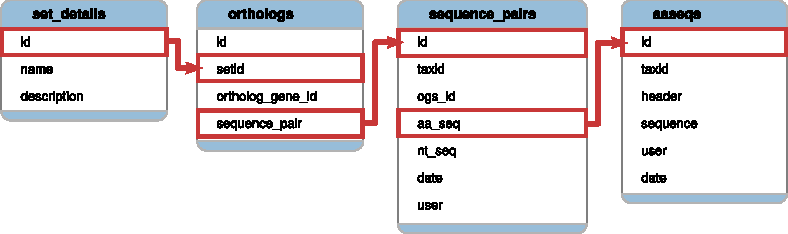
\includegraphics{img/db-orthoset.pdf}
	\caption[Database table connections for a given ortholog set]{
		\pname database structure for a given ortholog set. Each rounded rectangle
		represents a table with named columns. The red path delineates the
		\code{JOIN} query structure that returns all amino acid sequences (stored in
		the table ``aaseqs'') that belong to a given ortholog set. Ortholog set
		information is stored in the table ``set\_details''.
	}
	\label{fig:db-orthoset}
\end{figure}


\begin{figure}[ht]
	\centering
	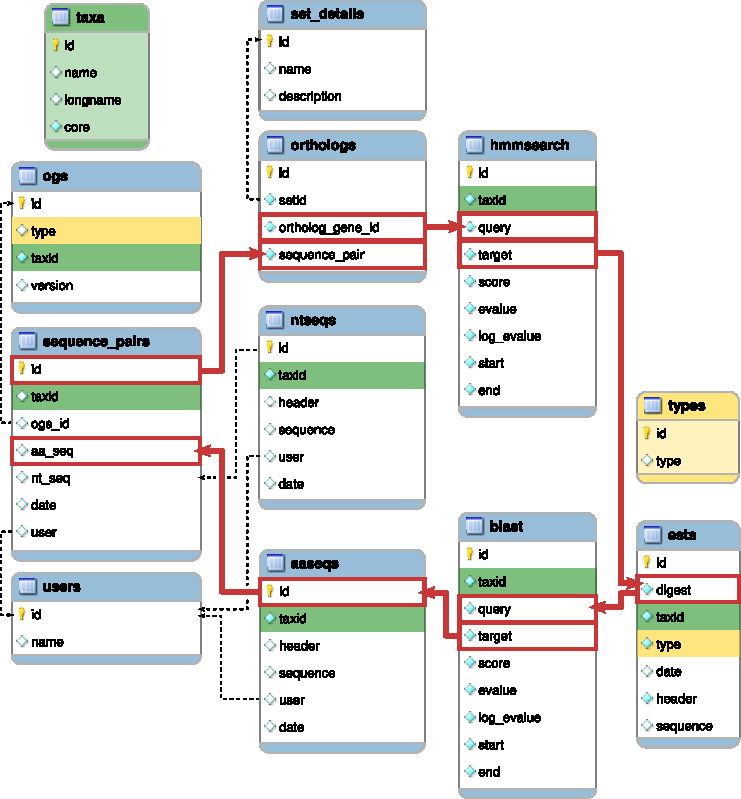
\includegraphics[width=\textwidth]{img/dbstructure.pdf}
	\caption[\pname database structure]{
		\pname database structure. Each rectangle represents a table with named
		columns. Note the circular path (red) that can be drawn across the tables and
		that is used in \code{JOIN} queries in order to construct a graph of
		orthologous relationships. Green table columns are referenced to the ``taxa''
		table, and yellow table columns are referenced to the ``types'' table. Dotted
		lines are secondary references.
	}
	\label{fig:dbstructure}
\end{figure}




	\section{Performance tweaks}
		\subsection{One BLAST database comprising all core taxa proteomes}
			\pname uses a single BLAST database comprising all reference taxa proteomes.
Only one BLAST search is performed for each HMM hit.

		\subsection{RBDMS vs. flat files}
		\subsection{MySQL performance}
	\section{SHA-256 checksums as sequence identifiers}
		Unique sequence IDs are necessary in order for \code{hmmsearch} not to create
confusion by treating whitespace in sequence headers as a description
separator. To avoid this, and to maintain a consistent naming scheme across
applications, \pname~uses a SHA-256 checksum to generate a unique ID for every
sequence. The checksum is generated using both the original header and the
sequence. Sequences are loaded into the database along with these checksums.
During the analysis, wherever a file is generated that includes sequence
identifiers, this checksum is used. This also eliminates the problem with
\code{fastatranslate} introducing whitespace that might confuse
\code{hmmsearch}.

It must be guaranteed that no two checksums, i.e., two sequence identifiers, are
ever the same. The SHA-256 hashing algorithm generates a checksum that is 160 bits,
or 40 hexadecimal characters in length. The probability $p$ of a hash collision
(i.e., two hashed elements returning the same checksum) in $n$ elements is

\begin{equation}
p \ge \frac{n (n-1)}{2} \times \frac{1}{2^b}
\label{eq:hashcollision}
\end{equation}

where $b$ is the number of bits generated by the hash function. There need to be
more than $1.7 \times 10^{15}$ objects for the SHA-256 hashes to exceed a collision
probability of $10^{-18}$. Since the hash space is expected to contain only a
number of objects in the range of $10^6$ to $10^{12}$, it is statistically safe
to assume that every checksum is unique. 



	\section{Benchmarks}
	\section{HMM sensitivity}

\chapter{Discussion and outlook}
	The results are of theoretical and practical nature and shed light on how a
pipeline for orthology prediction using HMMs and a RDBMS should be designed,
including challenges and pitfalls. 
The results also highlight the high potential of an extensive, metadata-enriched
ortholog cluster graph for phylogenetic and other analyses. 

During the development of \pname, I was faced with obstacles of both theoretical
and practical nature. I gained insights into the delicacies of modern Perl
development and high-performance MySQL database implementations.

	\section{Summary}
	\section{Outlook}
\clearpage

\section{Methodology}
\clearpage

\section{Comparisons with \hamstr}
\clearpage

\section{Conclusion and outlook}
\clearpage

\phantomsection
\addcontentsline{toc}{chapter}{Bibliography}
\bibliographystyle{plainnat}
\bibliography{bib/diploma}
\clearpage

\phantomsection
\addcontentsline{toc}{chapter}{List of figures}
\listoffigures
\clearpage

\phantomsection
\addcontentsline{toc}{chapter}{List of tables}
\listoftables
\clearpage

\phantomsection
\appendix
\chapter{Appendix}
	\section{Listings}
		%\lstinputlisting[caption=Inserting random nucleotides at random intervals at a given probability, label=lst:randomframeshifts]{scripts/insertrandomframeshifts.pl}


\phantomsection
\chapter*{Acknowledgements}
	I thank Bernhard Misof for commiting this project to me, for helpful comments
and for maintaining such a great atmosphere in this working group.

Thanks to Oliver Niehuis for really good supervising and helpful discussions.
Your challenges made me outgrow my own boundaries.

I also thank Karen Meusemann for being a brilliant office-mate, for interesting
discussions, and for forming a great team. You made my diploma year.

Thanks to Alex Donath, Julia Schwarzer, Sandra Meid, Patrick Kück, Caro Greve,
Ralph Peters, Christoph Mayer, Jeanne Wilbrandt, Tanja Ziesmann, and Hannes
Jäkel for contributing to a good working group. Without all of you this year
wouldn't have been the same.

I also acknowledge Torsten Struck, who was the first to point out the redundant
assignment bug in \hamstr, and the helpful programming community at
\url{stackoverflow.com}, which helped me with tough questions concerning Perl
and MySQL, as well as Peter Grobe, whose concrete advice helped in designing the
database.

Thanks to Silvio Philipp as well as Alf and Monika Sibla for their friendship
and for taking my mind off everything else for a few hours each Wednesday. 

Many thanks to Hannah for making me smile every day, taking care of everything
and enduring my absent-mindedness the last few weeks. 

	\clearpage

\phantomsection
\addcontentsline{toc}{chapter}{Declaration of authorship}
\chapter*{Declaration of authorship}
	Ich versichere hiermit an Eides statt, dass die vorliegende Diplomarbeit
selbstständig verfasst und keine weiteren als die angegebenen Hilfsmittel
benutzt sowie die Stellen der Arbeit, die in anderen Werken dem Wortlaut oder
dem Sinn nach entnommen sind, durch Angaben der Quellen sichtbar gemacht
wurden.

\vspace{4em}

\parbox[t]{0.3\textwidth}{\dotfill}

Bonn, \today

\vspace{8em}

\author

\end{document}
